\begin{center}
  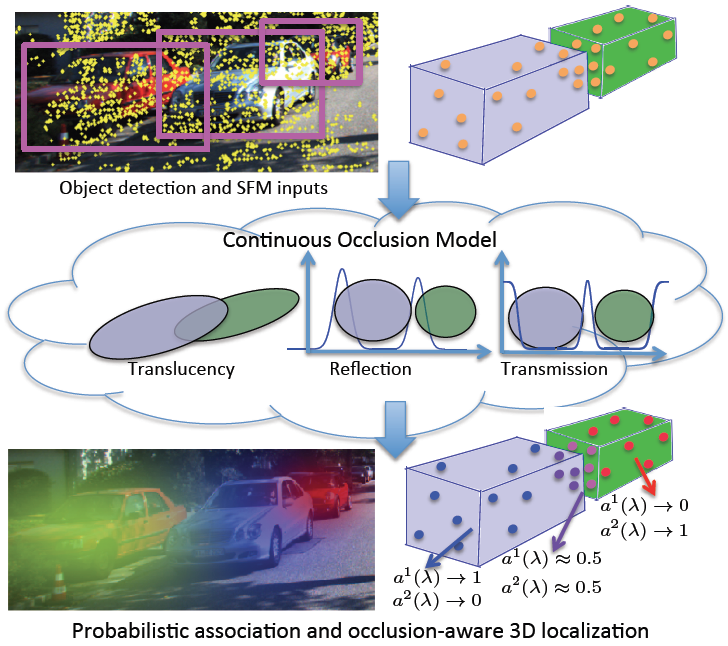
\includegraphics[width=\linewidth]{graphics/figure1.png}
\end{center}
\vspace{-0.6cm}
\caption{\small We propose an occlusion model in 3D that is physically-inspired and continuous. Given object detection and SFM point tracks, our unified model probabilistically assigns point tracks to objects and reasons about object detection scores and bounding boxes. It uniformly handles static and dynamic objects, thus, outperforms motion segmentation for association problems. We also demonstrate occlusion-aware 3D localization in road scenes.}
\label{fig:page1}
